\documentclass[11pt,ngerman]{article}
\usepackage[utf8]{inputenc}
%?
\linespread{1.0}
\setlength{\parskip}{0.7em}
\setlength{\baselineskip}{0.2cm}
\setlength{\parindent}{0em}
\usepackage[a4paper,left=2cm,right=2cm,top=2cm,bottom=2cm,bindingoffset=5mm]{geometry}
%?
\usepackage{hyperref}
\usepackage{booktabs}
\usepackage{graphicx}

\begin{document}
\title{Summary Computer Networks}
\author{John}
\maketitle

\tableofcontents



\section{Motivation}

\subsection{Communication	Metaphors}
\begin{itemize}
	\item Phase 1: Person to person
	\item Phase 2: Person to machine
	\item Phase 3: Machine to machine/Network of computers
	\item Phase 4: The internet of Things
\end{itemize}

\subsection{History}
\begin{itemize}
	\item 1837:	Samuel	Morse	develops	the	telegraph
	\item 1953:	First	transatlantic	Telephone	line
	\item 1876:	Alexander	Graham	Bell	patents	the	telephone	(tele=distant,	phone=voice)
\end{itemize}

\subsection{Telephone	Network}
Existing	networks	are	going	to	be	integrated\\
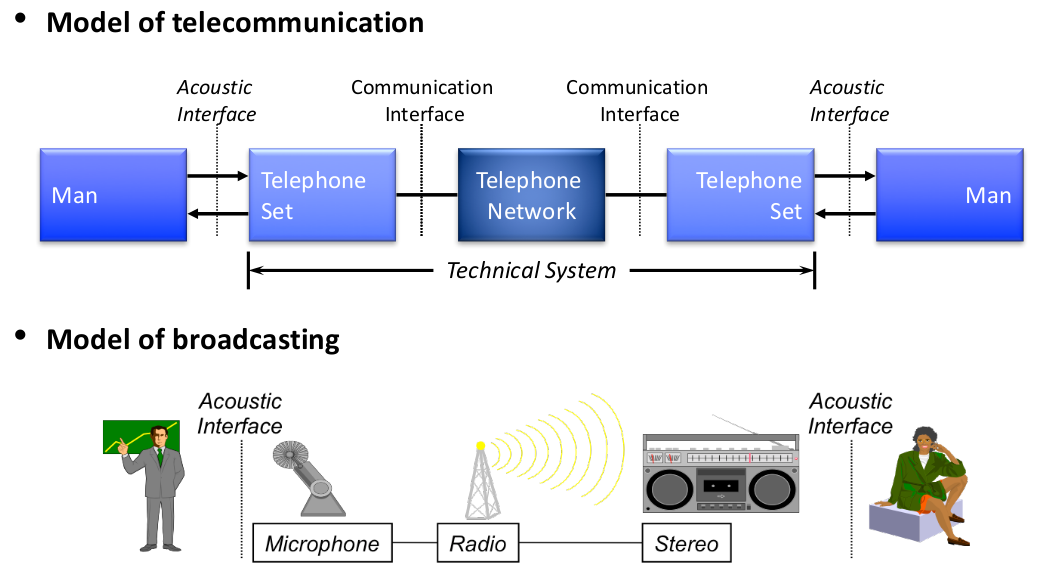
\includegraphics[width=5in]{images/Selection_001.png}

\subsection{The Internet}7
The internet consists of
\begin{itemize}
	\item a	set	of	computers,	which
	\begin{itemize}
		\item use	the	TCP/IP	protocols
		\item are	somehow	(directly	or	indirectly)	connected
		\item offer	or	use	particular	services
	\end{itemize}
	\item a	set	of	users,	which	have	access	to	these	services
	\item a	set	of	other	networks,	which	(somehow)	are	accessible
\end{itemize}

Design Principles
\begin{itemize}
	\item Minimalism	and	autonomy  - The	network	operates	by	itself	, does	not	require	internal	changes	when	new	networks	are	added
	\item Best-effort	service	model
	\item Soft-state	(stateless) - The	routers	do	not need	to	maintain end-to-end	communication	
information
	\item Decentralization
\end{itemize}



%%%%%%%%%%%%%%%%%%%%%%%%%%%%%%%%%%%%%%%%%%%%%%%%%%%%%%%%%%



\section{Introduction}
\subsection{Data	Communication}
Data	communication	is	the	processing	and	the	transport	of	digital	data	over	
connections	between	computers	(generally	over	large	distances).\\
Data	communication	comprises	two areas: Computer	Networks and Communication	Protocols

\subsection{What	is	Digital	Data?}
\begin{itemize}
	\item Data: Representation	of	facts in	a	formal	way, processable by humans and machines, e.g. a language
	\item Information:  is	whatever	contributes	
to	a	reduction	in	the	uncertainty	of	the	state	of	a	system, can only be handled by humans
	\item Signal: is	the	physical	representation	
of	data	by	spatial	or	timely	variation	
of	physical	characteristics
	\item Example:  Sounds	of	a	language	(Data)	during	speaking	are	acoustic	waves	(Signals)
\end{itemize}

\subsection{Data	Communication}
\begin{itemize}
	\item Sharing	resources	saves	costs
	\item Exchange	of	information
\end{itemize}

\subsection{Networking	Principles}
Communication	Peers
\begin{itemize}
	\item Unicast:	Two	communication	peers	
communicate	over	a	Point-to-Point	
connection.
	\item Multicast:	One	sender	
communicates	to	several	receivers,	
which	are	known.
	\item Broadcast:	One	sender	transmits	to	
all	other	peers.
Typically	the	other	peers	are	
(partially)	unknown.
	\item Others:	Anycast,	Geocast,	etc.
\end{itemize}

Transmission
\begin{itemize}
	\item Serial Transmission
	\item Parallel Transmission (Problem: synchronisation of the data)
	\item Asynchronous Transmission:	Transmission	in	which	each	block	
(character)	is	individually	synchronized\\
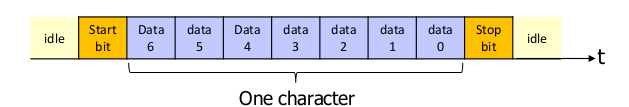
\includegraphics[width=5in]{images/Selection_002.png}

	\item Synchronous Transmission:	Transmission	in	which	the	time	of	
occurrence	of	each	signal	representing	a	bit	is	related	to	a	fixed	time	
frame \\
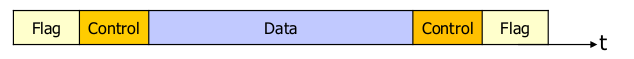
\includegraphics[width=5in]{images/Selection_003.png}
\end{itemize}

Connection	Properties\\
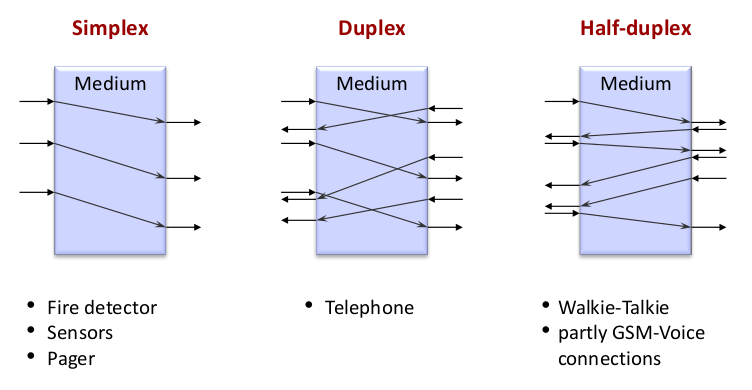
\includegraphics[width=5in]{images/Selection_004.png}

Multiplexing:
Combining	multiple	data	
channels	into	a	single	data	
channel	at	the	source\\

Quality\\
\begin{itemize}
	\item Technical	Performance (Delay-Bandwidth-Product	=	
Store	capacity of	the	line)
	\begin{itemize}
		\item Delay	[s]
		\item Jitter	[s]
		\item Throughput	[bit/s]
		\item Data	rate	[bit/s] (wird vorgegeben)
	\end{itemize}
	\item Costs
	\item Reliability
	\item Security	and	Protection\\
		Safety measures: Encryption, Trustworthy	systems	\\
	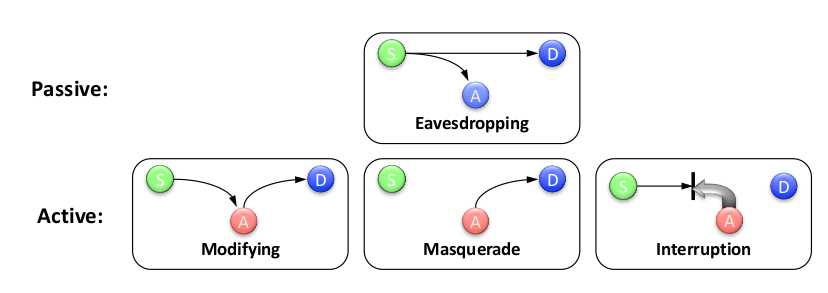
\includegraphics[width=5in]{images/Selection_005.png}
\end{itemize}


The	Client/Server	Principle
\begin{itemize}
	\item Client $\rightarrow$ Server: Request
	\item Server $\rightarrow$ Client: Reply 
\end{itemize}
\begin{itemize}
	\item Advantages
	\begin{itemize}  
	\item Cost	reduction
	\item Better	usage	of	resources
	\item Modular	extensions
	\item Reliability	by	redundancy
	 \end{itemize}
	\item Server: Program	(process)	which	offers	a	service	over	a	network.	
	\item Client: Program	(process)	which	uses	a	service	offered	by	a	server.
\end{itemize}


Peer-to-Peer	Principle (ursprüngliche Kommunikation im Internet)
\begin{itemize}
	\item Equal	partners,	no	fixed	client	and	server	roles
	\item Connections	between	any	pair	of	computers
	\item Establishment	of	a	whole	network	of	connections
	\item Best	example:	File	Sharing,	e.g.,	Napster,	Gnutella
\end{itemize}

\subsection{Communication	Protocols}
WHY Protocol!	
\\\\
A	protocol	is	the	set	of	agreements	between	(application)	processes	with	the	purpose	of	
communication.\\
	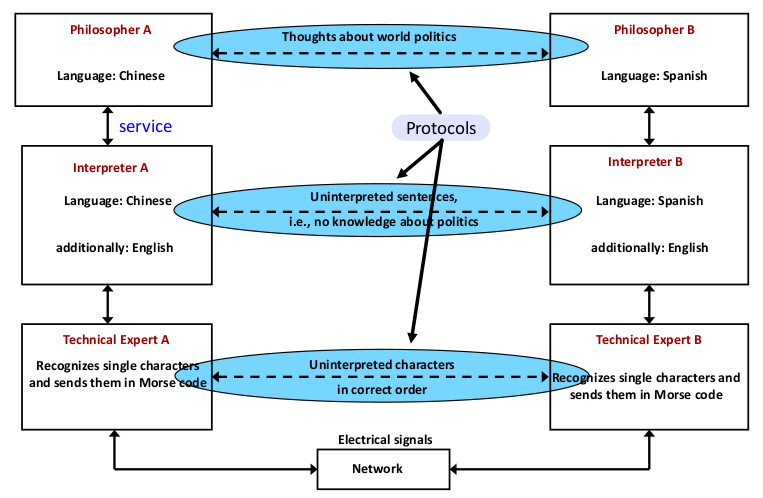
\includegraphics[width=5in]{images/Selection_006.png}\\
	$\rightarrow$ communication between horizontal layers
	
Peer	of	a	Layer
\begin{itemize}
\item
use	one	service	
(except	the	bottom)
\item
offer	a	service	
(except	the	top)
\item
do	not	need	to	know	other	
than	the	next	lower	one
\item
talk	according	to	the	rules
\end{itemize}

Communication	architectures	are	based	on
\begin{itemize}
\item  Service	=	Communication	Service
\item Rules	=	Communication	Protocol

\end{itemize}


\end{document}

Model	of	layers	is	applied	to	simplify	the	complexity
•
•
ISO/OSI
TCP/IP
There	are	many	global	players	in	computer	networking
•
Standardization
Computer	networks
•
Different	kinds	of	computer	networks	exist